\documentclass[a4paper,twoside,onecolumn,openany,article,10pt]{memoir}
\usepackage{xeCJK}
\usepackage{url}
\usepackage{hyperref}
\usepackage{amsmath}
\usepackage{amssymb}
\usepackage{amsthm}
\usepackage{enumerate}
\usepackage{algorithm}
\usepackage{algorithmicx}
\usepackage{algpseudocode}
\usepackage{ascmac}
\usepackage{tikz}
%\usepackage{stix}
\defaultfontfeatures{Ligatures=TeX}

\setCJKmainfont[BoldFont=Noto Sans CJK JP]{Noto Serif CJK JP}
\setCJKsansfont{Noto Sans CJK JP}
%\setCJKmonofont{Noto Mono CJK JP}

\newtheorem{theorem}{定理}
\theoremstyle{remark}
\newtheorem{remark}{\textbf{余談}}


\setmainfont{DejaVu Serif}
%\setsansfont{URW Gothic}
\setmonofont{Inconsolata}

\usepackage{listings}

%\renewcommand{\algorithmcfname}{アルゴリズム}



\settrimmedsize{\stockheight}{\stockwidth}{*}

%\setlrmarginsandblock{1.5in}{1in}{*}
\setlrmarginsandblock{1.2in}{1.2in}{*}
\setulmarginsandblock{1.2in}{1.5in}{*}
\setheadfoot{20mm}{15mm}

%\newlength{\linespace}
%\setlength{\linespace}{\baselineskip}
%\setlength{\headheight}{\onelineskip}
%\setlength{\headsep}{\linespace}
%\addtolength{\headsep}{-\topskip}

%\setlength{\footskip}{\onelineskip}
%\setlength{\footnotesep}{\onelineskip}

\checkandfixthelayout

\counterwithout{section}{chapter}
\setsecnumdepth{subsubsection}


\title{アルゴリズムとデータ構造~レポート1~プログラミング演習}
\date{2017年6月27日}
\author{森~立平 \texttt{mori@c.titech.ac.jp}}

\begin{document}
\maketitle

\section{レポート1のプログラミング課題の補足説明}
\if0
\subsection{課題}
各問題に対して動的計画法を設計せよ。
各問題について
\begin{itemize}
\item 補助関数の定義
\item 補助関数の満たす再帰的な関係式
\item 補助関数から問題の解を計算する方法
\item アルゴリズム全体の説明
\item 時間計算量、空間計算量の評価
\end{itemize}
をA4レポート用紙両面1枚に記入せよ(難易度$\bigstar\bigstar\bigstar$については枚数制限はない)。
\fi

\subsection{実行時間と入力制約}
各問題には入力制約がある。大雑把に言って、$O(f(n))$時間アルゴリズムであれば、$f(n)\le 10^7$となる $n$については、大体どのような実行環境でも1秒以内に計算が終わる。
大体の目安として
\begin{itemize}
\item $n\le 200$ は $O(n^3)$ 時間アルゴリズムで1秒以内に解ける。
\item $n\le 1000$ は $O(n^2)$ 時間アルゴリズムで1秒以内に解ける。
\item $n\le 10^5$ は $O(n\log n)$ 時間アルゴリズムで1秒以内に解ける。
\item $n\le 10^7$ は $O(n)$ 時間アルゴリズムで1秒以内に解ける。
\item $n\le 10^{18}$ は $O(\log n)$ 時間アルゴリズムで一瞬で解ける。
\end{itemize}
もちろん、オーダーはあくまで漸近的な尺度なのでこれらは目安にすぎない。
同じオーダーの時間計算量でもプログラムの実装によってプログラムの実行速度は大きく変わり得る。

この課題で各問題について設計する動的計画法は
演習室で実行したときに
入力制約を満たす任意の入力に対して
1秒以内に計算が終了するものでなくてはならない。
想定している通りの解法であれば、どのような実装でも十分間に合う。
実行時間を計るには \texttt{time ./a.out < input.txt} とコマンドの先頭に \texttt{time} をつければよい。

\subsection{注意点}
\begin{itemize}
\item 最適解を求める問題では複数存在しうる最適解のうちの1つを出力すればよい。
\item 配列のサイズを\texttt{N}とすると、\texttt{dp[0], ..., dp[N-1]} を使用することができる。
もしも\texttt{dp[N]}まで使用したいのであれば、配列のサイズを\texttt{N+1}にする必要がある。
\item プログラムで入力を受け取る際には\texttt{scanf}を用いる。
整数を一つ受け取り変数\texttt{n}に代入したい場合は\texttt{scanf("\%d", \&n);}とする。
二つの整数を受け取り変数\texttt{n, m}にこの順番で代入したい場合は
\texttt{scanf("\%d\%d", \&n, \&m);}とする。
配列に値を代入する場合も同様であるが\texttt{\&A[i]}の代わりに\texttt{A+i}が使える。
この\texttt{scanf}は空白や改行は適宜飛ばして読むので、入力に含まれる改行について考慮する必要はない。
\end{itemize}

\clearpage
\section{問題}
\if0
\subsection{分割数}
\begin{itembox}[l]{問題文}
$n$を自然数を用いて分割する方法の数を$10^9$で割った余り$X$を求めよ。
\end{itembox}

\begin{itembox}[l]{入力制約}
$1\le n\le 1000$
\end{itembox}

\begin{itembox}[l]{入力}
$n$
\end{itembox}

\begin{itembox}[l]{出力}
$X$
\end{itembox}

\begin{itembox}[l]{サンプル1}
入力:
\begin{verbatim}
8
\end{verbatim}
出力:
\begin{verbatim}
22
\end{verbatim}
\end{itembox}

\begin{itembox}[l]{サンプル2}
入力:
\begin{verbatim}
100
\end{verbatim}
出力:
\begin{verbatim}
190569292
\end{verbatim}
\end{itembox}

\begin{itembox}[l]{サンプル3}
入力:
\begin{verbatim}
200
\end{verbatim}
出力:
\begin{verbatim}
999029388
\end{verbatim}
\end{itembox}

\begin{itembox}[l]{サンプル4}
入力:
\begin{verbatim}
1000
\end{verbatim}
出力:
\begin{verbatim}
149727991
\end{verbatim}
\end{itembox}

\clearpage
\subsection{与えられた整数を用いた分割の総数}
\begin{itembox}[l]{問題文}
与えられた $A=\{a_1,\dotsc,a_m\}$ と $n$ について、
$n$を$A$に含まれる自然数のみを用いて分割する方法の数を$10^9$で割った余り$X$を求めよ。
\end{itembox}

\begin{itembox}[l]{入力制約}
$1\le n\le 1000$\\
$1\le m\le 1000$\\
$1\le a_i \le n, \qquad\forall i\in\{1,\dotsc,m\}$\\
$a_i$ は互いに異なる。
\end{itembox}

\begin{itembox}[l]{入力}
$n\quad m$\\
$a_1\, \cdots\, a_m$
\end{itembox}

\begin{itembox}[l]{出力}
$X$
\end{itembox}

\begin{itembox}[l]{サンプル1}
入力:
\begin{verbatim}
8 8
1 2 3 4 5 6 7 8
\end{verbatim}
出力:
\begin{verbatim}
22
\end{verbatim}
\end{itembox}

\begin{itembox}[l]{サンプル2}
入力:
\begin{verbatim}
100 3
1 3 5
\end{verbatim}
出力:
\begin{verbatim}
364
\end{verbatim}
\end{itembox}

\begin{itembox}[l]{サンプル3}
入力:
\begin{verbatim}
101 1
2
\end{verbatim}
出力:
\begin{verbatim}
0
\end{verbatim}
\end{itembox}
\fi

\subsection{最適な行列積の順番 $\bigstar$}
\begin{itembox}[l]{問題文}
各$i=1,2,\dotsc,n$について$M_i$を$a_i\times a_{i+1}$行列としたとき、
行列積$M_1M_2\dotsm M_{n}$を計算するための最小のスカラー乗算回数$X$をもとめよ。
ただし、$a\times b$行列と$b\times c$行列の行列積には$abc$回のスカラー乗算が必要とする。
\end{itembox}

\begin{itembox}[l]{入力制約}
$1\le n\le 100$\\
$1\le a_i\le 100,\quad\forall i\in\{1,\dotsc,n+1\}$
\end{itembox}

\begin{itembox}[l]{入力}
$n$\\
$a_1\, \cdots\, a_{n+1}$
\end{itembox}

\begin{itembox}[l]{出力}
$X$
\end{itembox}

\begin{itembox}[l]{サンプル1}
入力:
\begin{verbatim}
3
1 2 3 4
\end{verbatim}
出力:
\begin{verbatim}
18
\end{verbatim}
説明:

\vspace{.5em}
最初に$1\times 2$行列と$2\times 3$行列の積を計算する(スカラー乗算6回)。それから$1\times 3$行列と$3\times 4$行列の積を計算する(スカラー乗算12回)。
するとスカラー乗算は合計で18回となる。
先に$2\times 3$行列と$3\times 4$行列の行列積を計算すると、最初の行列積だけでスカラー乗算が24回必要となってしまう。
\end{itembox}

\begin{itembox}[l]{サンプル2}
入力:
\begin{verbatim}
10
2 4 3 7 9 8 2 3 4 7 8
\end{verbatim}
出力:
\begin{verbatim}
552
\end{verbatim}
\end{itembox}


\clearpage
\subsection{棒の価値 $\bigstar$}
\begin{itembox}[l]{問題文}
整数$i$について、長さ$i$の棒は$a_i$円で売れる。
長さ$i$の棒を2つにカットして長さ$j$の棒($1\le j< i$)と長さ$i-j$の棒を得るのに$k$円かかる。
長さ$n$の棒を使って上げることのできる利益の最大値$X$と対応する分割$(N_1, N_2, \dotsc, N_m)$を求めよ。
\end{itembox}

\begin{itembox}[l]{入力制約}
$1\le n\le 1000$\\
$0\le k\le 10^5$\\
$1\le a_i\le 10^5,\quad\forall i\in\{1,\dotsc,n\}$.
\end{itembox}

\begin{itembox}[l]{入力}
$n\quad k$\\
$a_1\, \cdots\, a_n$
\end{itembox}

\begin{itembox}[l]{出力}
$X$\\
$N_1\quad N_2\quad \dotsc\quad N_m$\\
(但し、$N_1\le N_2\le\dotsb \le N_m$ とする)
\end{itembox}

\begin{itembox}[l]{サンプル1}
入力:
\begin{verbatim}
5 1
1 2 3 4 2
\end{verbatim}
出力:
\begin{verbatim}
4
1 4
\end{verbatim}
\end{itembox}

\begin{itembox}[l]{サンプル2}
入力:
\begin{verbatim}
10 10
10 9 8 7 6 5 4 3 2 1
\end{verbatim}
出力:
\begin{verbatim}
10
1 1 1 1 1 1 1 1 1 1
\end{verbatim}
\end{itembox}


\clearpage
\subsection{最長共通部分数列 $\bigstar$}
\begin{itembox}[l]{問題文}
2つの数列 $a_1, a_2,\dotsc, a_n$ 
と $b_1, b_2,\dotsc, b_m$ の連続するとは限らない共通部分数列の最大の長さ$X$
とその共通部分数列$C_1, C_2,\dotsc, C_X$を求めよ。
\end{itembox}

\begin{itembox}[l]{入力制約}
$1\le n, m\le 1000$\\
$1\le a_i\le 10^9,\quad\forall i\in\{1,\dotsc,n\}$\\
$1\le b_i\le 10^9,\quad\forall i\in\{1,\dotsc,m\}$
\end{itembox}

\begin{itembox}[l]{入力}
$n\quad m$\\
$a_1\, \cdots\, a_n$\\
$b_1\, \cdots\, b_m$
\end{itembox}

\begin{itembox}[l]{出力}
$X$\\
$C_1\, \cdots\, C_X$
\end{itembox}

\begin{itembox}[l]{サンプル1}
入力:
\begin{verbatim}
4 3
1 2 4 3
1 2 3
\end{verbatim}
出力:
\begin{verbatim}
3
1 2 3
\end{verbatim}
\end{itembox}

\begin{itembox}[l]{サンプル2}
入力:
\begin{verbatim}
4 4
1 8 3 1
1 1 3 8
\end{verbatim}
出力:
\begin{verbatim}
2
1 8
\end{verbatim}
\end{itembox}

\clearpage
%\section{難易度$\bigstar\bigstar$}
\subsection{最大部分和$\bigstar\bigstar$}
\begin{itembox}[l]{問題文}
数列 $a_1, a_2,\dotsc, a_n$ の連続する部分数列 $a_{L}, a_{L+1},\dotsc, a_R$ の和の最大値$X$と対応する区間$[L,R]$を求めよ。
\end{itembox}

\begin{itembox}[l]{入力制約}
$1\le n\le 10^6$\\
$-1000\le a_i\le 1000,\quad\forall i\in\{1,\dotsc,n\}$
\end{itembox}

\begin{itembox}[l]{入力}
$n$\\
$a_1\, \cdots\, a_n$
\end{itembox}

\begin{itembox}[l]{出力}
$X$\\
$L$ $R$\\
(ただし空の区間は$L=R=0$で表すとする)
\end{itembox}

\begin{itembox}[l]{サンプル1}
入力:
\begin{verbatim}
5
1 1 1 1 1
\end{verbatim}
出力:
\begin{verbatim}
5
1 5
\end{verbatim}
\end{itembox}

\begin{itembox}[l]{サンプル2}
入力:
\begin{verbatim}
10
1 -2 3 -1 4 -5 8 -3 1 1
\end{verbatim}
出力:
\begin{verbatim}
9
3 7
\end{verbatim}
\end{itembox}

\begin{itembox}[l]{サンプル3}
入力:
\begin{verbatim}
3
-1 -1 -1
\end{verbatim}
出力:
\begin{verbatim}
0
0 0
\end{verbatim}
\end{itembox}

\clearpage
\subsection{ペアの作り方$\bigstar\bigstar$}
\begin{itembox}[l]{問題文}
1から$n$までの数字の中でペアをいくつか作りたい。
一つの数字は高々一つのペアに属している。
また、2つのペア$\{x_1, y_1\}$ と$\{x_2,y_2\}$について、
$x_1<x_2<y_1<y_2$となることが無いとする。
そのようなペア達の作り方の総数を$10^9$で割った余り$X$をもとめよ。
\end{itembox}

\begin{itembox}[l]{入力制約}
$1\le n\le 1000$
%\\$1\le n\le 10^6$ \hspace{2em}(難易度$\bigstar\bigstar\bigstar$)
\end{itembox}

\begin{itembox}[l]{入力}
$n$
\end{itembox}

\begin{itembox}[l]{出力}
$X$
\end{itembox}

\begin{itembox}[l]{サンプル1}
入力:
\begin{verbatim}
4
\end{verbatim}
出力:
\begin{verbatim}
9
\end{verbatim}
説明:

\vspace{.5em}
$\varnothing$\\
\{1,2\}\\
\{2,3\}\\
\{3,4\}\\
\{1,3\}\\
\{2,4\}\\
\{1,4\}\\
\{1,2\}, \{3,4\}\\
\{1,4\}, \{2,3\}\\
の9通り。
\end{itembox}

\noindent
\begin{minipage}[t]{0.33\hsize}
\begin{itembox}[l]{サンプル2}
入力:
\begin{verbatim}
5
\end{verbatim}
出力:
\begin{verbatim}
21
\end{verbatim}
\end{itembox}
\end{minipage}
\begin{minipage}[t]{0.33\hsize}
\begin{itembox}[l]{サンプル3}
入力:
\begin{verbatim}
100
\end{verbatim}
出力:
\begin{verbatim}
193303669
\end{verbatim}
\end{itembox}
\end{minipage}

\clearpage
\subsection{最短経路の数$\bigstar\bigstar$}
\begin{itembox}[l]{問題文}
$h\times w$ のマス目がある。
マス目は\#で表わされるものと.で表わされるものがある。
あるマス目からその上下左右のマス目に移動することができるが\#のマス目には移動できない。
左上のマス目からスタートして右下のマス目に$h+w-2$回の移動で到達する方法の数を$10^9$で割った余り$X$を答えよ。
\end{itembox}

\begin{itembox}[l]{入力制約}
$1\le h, w\le 1000$\\
$2\le h+w$
\end{itembox}

\begin{itembox}[l]{入力}
$h$ $w$\\
$c_{1,1} \dotsb c_{1,w}$\\
$\vdots$\\
$c_{h,1} \dotsb c_{h,w}$\\
(各$c_{i,j}$は\#か.のいずれかである。)\\
($c_{1,1} = c_{h,w} = .$)
\end{itembox}

\begin{itembox}[l]{出力}
$X$
\end{itembox}

\noindent
\begin{minipage}[t]{0.33\hsize}
\begin{itembox}[l]{サンプル1}
入力:
\begin{verbatim}
3 3
...
...
...
\end{verbatim}
出力:
\begin{verbatim}
6
\end{verbatim}
\end{itembox}
\end{minipage}
\begin{minipage}[t]{0.33\hsize}
\begin{itembox}[l]{サンプル2}
入力:
\begin{verbatim}
4 3
...
.#.
.#.
...
\end{verbatim}
出力:
\begin{verbatim}
2
\end{verbatim}
\end{itembox}
\end{minipage}
\begin{minipage}[t]{0.33\hsize}
\begin{itembox}[l]{サンプル3}
入力:
\begin{verbatim}
5 5
.....
###..
.....
..###
.....
\end{verbatim}
出力:
\begin{verbatim}
0
\end{verbatim}
\end{itembox}
\end{minipage}

\begin{itembox}[l]{サンプル4}
入力:
\begin{verbatim}
5 80
................................................................................
................................................................................
.......................................#........................................
................................................................................
................................................................................
\end{verbatim}
出力:
\begin{verbatim}
1131600
\end{verbatim}
\end{itembox}

%\clearpage
%\subsection{連続する$k$個の0/1を持たない01列の数}

\clearpage
%\section{難易度$\bigstar\bigstar\bigstar$}

\if0
\subsection{最長単調非減少列}
\begin{itembox}[l]{問題文}
数列 $a_1, a_2,\dotsc, a_n$ の連続するとは限らない単調非減少な部分数列で最長なもの$a_{i_1}, \dotsc, a_{i_X}$とその長さ$X$を求めよ。
\end{itembox}

\begin{itembox}[l]{入力制約}
$1\le n\le 1000$\\
$1\le n\le 10^6$\hspace{2em} (難易度$\bigstar\bigstar\bigstar\bigstar$)\\
$1\le a_i\le 10^9,\quad\forall i\in\{1,\dotsc,n\}$
\end{itembox}

\begin{itembox}[l]{入力}
$n$\\
$a_1,\dotsc,a_n$
\end{itembox}

\begin{itembox}[l]{出力}
$X$\\
$a_{i_1} \dotsb a_{i_X}$
\end{itembox}

\begin{itembox}[l]{サンプル1}
入力:
\begin{verbatim}
10
10 2 3 8 7 2 9 1 11 3
\end{verbatim}
出力:
\begin{verbatim}
5
2 3 7 9 11
\end{verbatim}
\end{itembox}

\begin{itembox}[l]{サンプル2}
入力:
\begin{verbatim}
10
10 9 8 7 6 5 4 3 2 1
\end{verbatim}
出力:
\begin{verbatim}
1
7
\end{verbatim}
\end{itembox}
\fi

%\clearpage
%\subsection{行列積の括弧の付け方}

\if0
\clearpage
\subsection{べき乗和の公式}
\begin{itembox}[l]{問題文}
非負整数$k=0, 1,2,\dotsc$について関数$S_k(n)$を
\begin{equation*}
S_k(n) := \sum_{i=1}^n x^k
\end{equation*}
と定義する。
$k=0,1,2$については
\begin{align*}
S_0(n) &= n\\
S_1(n) &= \frac{n(n+1)}2 = \frac{n^2 + n}2\\
S_2(n) &= \frac{n(n+1)(2n+1)}6 = \frac{2n^3 + 3n^2 + n}2
\end{align*}
が成り立つ。
一般の$k$について$S_k(n)$は$n$の$k+1$次多項式になる。
与えられた$k$について$S_k(n)$の多項式表現
\begin{equation*}
S_k(n) = \frac{\sum_{i=1}^{k+1} a_i n^i}{m},\qquad \mathrm{gcd}(a_1,\dotsc,a_{k+1},m) = 1
\end{equation*}
をもとめよ。ここで$\mathrm{gcd}(x_1,\dotsc,x_t)$は整数$x_1,\dotsc,x_t$の最大公約数とする。
\end{itembox}

\begin{itembox}[l]{入力制約}
$0\le k\le 15$.
\end{itembox}

\begin{itembox}[l]{入力}
$k$
\end{itembox}

\begin{itembox}[l]{出力}
$a_{k+1}\quad  a_k\quad  \dotsc\quad  a_1$\\
$m$
\end{itembox}

\begin{itembox}[l]{サンプル1}
入力:
\begin{verbatim}
1
\end{verbatim}
出力:
\begin{verbatim}
1 1
2
\end{verbatim}
\end{itembox}

\begin{itembox}[l]{サンプル2}
入力:
\begin{verbatim}
10
\end{verbatim}
出力:
\begin{verbatim}
6 33 55 0 -66 0 66 0 -33 0 5
66
\end{verbatim}
\end{itembox}
\fi

\subsection{働き者$\bigstar\bigstar$}
\begin{itembox}[l]{問題文}
全部で$n$個の仕事がある。
$i$番目の仕事は時刻$a_i$に開始して時刻$b_i$の直前に終了し、$w_i$円の報酬がもらえる。
$n$個の仕事からいくつか選択して働いたときに得られる報酬の最大値$X$をもとめよ。
ただし、同時に複数の仕事はできないものとする。
また、時刻$b$の直前に終了する仕事の後に時刻$b$に開始する仕事をすることができるものとする。
\end{itembox}

\begin{itembox}[l]{入力制約}
$1\le n\le 1000$\\
$1\le n\le 10^5$ (難易度 $\bigstar\bigstar\bigstar$)\\
$1\le a_i < b_i\le 10^9\qquad \forall i\in\{1,\dotsc,n\}$\\
$a_i \le a_{i+1}\qquad \forall i\in\{1,\dotsc,n-1\}$\\
$1\le w_i \le 10^4\qquad \forall i\in\{1,\dotsc,n\}$
\end{itembox}

\begin{itembox}[l]{入力}
$n$\\
$a_1\ b_1\ w_1$\\
$\vdots$\\
$a_n\ b_n\ w_n$
\end{itembox}

\begin{itembox}[l]{出力}
$X$
\end{itembox}

\begin{itembox}[l]{サンプル1}
入力:
\begin{verbatim}
3
10 20 1
15 25 2
20 30 2
\end{verbatim}
出力:
\begin{verbatim}
3
\end{verbatim}
説明:

\vspace{.5em}
仕事1と仕事3を選ぶと報酬の合計が3円になる。
\end{itembox}

\begin{itembox}[l]{サンプル2}
入力:
\begin{verbatim}
3
10 20 1
15 19 2
20 30 2
\end{verbatim}
出力:
\begin{verbatim}
4
\end{verbatim}
\end{itembox}


\clearpage
\subsection{グリッド上のサイクルの数$\bigstar\bigstar\bigstar$}
\begin{itembox}[l]{問題文}
縦に4つ、横に$n+1$つ頂点が格子状に接続しているグラフ

\begin{center}
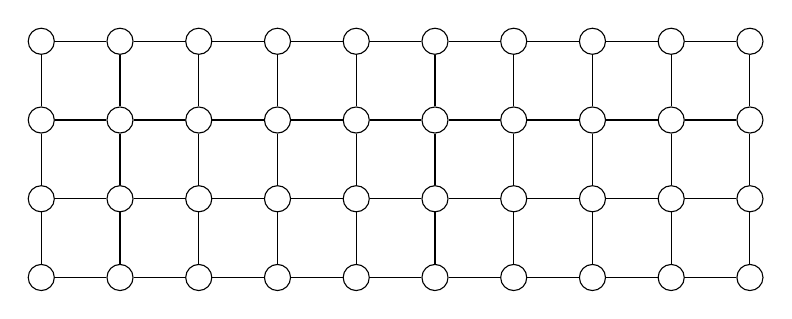
\begin{tikzpicture}
\foreach \x in {0,...,3}{
  \foreach \y in {0,...,9}{
    \node[circle,draw] (\y \x) at (\y, \x) {};
    \ifnum\y>0
      \pgfmathparse{int(\y-1)}
      \draw (\y \x) -- (\pgfmathresult \x);
    \fi
    \ifnum\x>0
      \pgfmathparse{int(\x-1)}
      \draw (\y \x) -- (\y \pgfmathresult);
    \fi
  }
}
\end{tikzpicture}
\end{center}
を$3\times n$のグリッドと呼ぶ。
$3\times n$ のグリッド上の単純閉路の個数を$10^9+7$で割った余り$X$をもとめよ。
\end{itembox}

\begin{itembox}[l]{入力制約}
$1\le n\le 10^6$\\
$1\le n\le 10^{18}$ (難易度 $\bigstar\bigstar\bigstar\bigstar$)
\end{itembox}

\begin{itembox}[l]{入力}
$n$
\end{itembox}

\begin{itembox}[l]{出力}
$X$
\end{itembox}

\begin{itembox}[l]{小さな$n$について}
$n=1,2,\dotsc,10$については
\begin{verbatim}
6, 40, 213, 1049, 5034, 23984, 114069, 542295, 2577870, 12253948
\end{verbatim}
\end{itembox}

\noindent
\begin{minipage}[t]{0.33\hsize}
\begin{itembox}[l]{サンプル1}
入力:
\begin{verbatim}
100
\end{verbatim}
出力:
\begin{verbatim}
652583913
\end{verbatim}
\end{itembox}
\end{minipage}
\begin{minipage}[t]{0.33\hsize}
\begin{itembox}[l]{サンプル2}
入力:
\begin{verbatim}
1000000
\end{verbatim}
出力:
\begin{verbatim}
595248477
\end{verbatim}
\end{itembox}
\end{minipage}
\begin{minipage}[t]{0.33\hsize}
\begin{itembox}[l]{サンプル3}
入力:
\begin{verbatim}
1000000000000000000
\end{verbatim}
出力:
\begin{verbatim}
103670646
\end{verbatim}
\end{itembox}
\end{minipage}


\end{document}
